\documentclass[]{aiaa-tc}% insert '[draft]' option to show overfull boxes

 \usepackage{varioref}%  smart page, figure, table, and equation referencing
 \usepackage{wrapfig}%   wrap figures/tables in text (i.e., Di Vinci style)
 \usepackage{threeparttable}% tables with footnotes
 \usepackage{dcolumn}%   decimal-aligned tabular math columns
  \newcolumntype{d}{D{.}{.}{-1}}
 \usepackage{nomencl}%   nomenclature generation via makeindex
  \makeglossary
 \usepackage{subfigure}% subcaptions for subfigures
 \usepackage{subfigmat}% matrices of similar subfigures, aka small mulitples
 \usepackage{fancyvrb}%  extended verbatim environments
  \fvset{fontsize=\footnotesize,xleftmargin=2em}
 \usepackage{lettrine}%  dropped capital letter at beginning of paragraph
 \usepackage[export]{adjustbox}
 \usepackage{url}

 \title{GPU acceleration of wall distance calculation for
   computational fluid dynamics codes}
 \author{
   Nathan A. Wukie\thanks{Graduate student researcher, School of Aerospace Systems, ML 70, 
     Cincinnati, OH, AIAA Student Member.}\\
   {\normalsize\itshape
     University of Cincinnati, Cincinnati, OH, 45221, USA}\\\\
   \ Chris Park\thanks{Software Engineer, GE Aviation} ,
   \ Vasanth Ganapathy\thanks{Lead Engineer, GE Aviation} \\
   {\normalsize\itshape
     GE Aviation, Cincinnati, OH, 45215 USA}\\
 }

 % Data used by 'handcarry' option
 %\AIAApapernumber{YEAR-NUMBER}
 %\AIAAconference{Conference Name, Date, and Location}
 %\AIAAcopyright{\AIAAcopyrightD{YEAR}}

 % Define commands to assure consistent treatment throughout document
 \newcommand{\eqnref}[1]{(\ref{#1})}
 \newcommand{\class}[1]{\texttt{#1}}
 \newcommand{\package}[1]{\texttt{#1}}
 \newcommand{\file}[1]{\texttt{#1}}
 \newcommand{\BibTeX}{\textsc{Bib}\TeX}

% Add highlighting - Wukie
\usepackage{color,soul}

\begin{document}

\maketitle

%\begin{abstract}
%Insert abstract
%\end{abstract}

%\section*{Nomenclature}

%\begin{tabbing}
%  XXX \= \kill% this line sets tab stop
%  $\rho$ \> Density \\
%  $\delta(f)$ \> Dirac delta function \\
%  $H(f)$ \> Heaviside function\\
%  $T_{ij}$ \> Lighthill stress tensor \\
%  $P_{ij}$ \> Compressive stress tensor \\
%  $u$ \> X-velocity \\
%  $v$ \> Y-velocity \\
%  $p'$ \> Pressure fluctuation\\
%  $x$ \> Tensor coordinate\\
%  $t$  \> Time\\
%  $c_o$ \> Reference speed of sound\\[5pt]
%  \textit{Subscript}\\
%  $i,j$ \> Tensor indices \\
%  $n$ \> Normal component\\
% \end{tabbing}

\section{Introduction}
\lettrine[nindent=0pt]{C}{omputational} fluid dynamics(CFD) is a branch of
simulation sciences that focuses on predicting fluid flows based on a
set of governing physical equations. There are many different methods
for accomplishing this that span both, different sets of governing
equations, in addition to different numerical methods for computing a
solution. Some different sets of equations that can be solved include
the potential flow equation, streamfunction-vorticity equations, Euler
equations, and Navier-Stokes equations. Analytical solutions to these
sets of equations are often not available except in some extremely
simple cases. Interesting geometries require a discretized
approach. Some common discretization methods include Finite Difference,
Finite Volume, and Finite Element methods. 

This research effort is focused on a problem for a subset
of those methods. In particular, we are interested in efficient wall
distance calculation algorithms to support Reynolds-Averaged
Navier-Stokes(RANS) solvers using a cell-centered, Finite Volume discretization with a
moving mesh capability.

\subsection{Background}

\subsubsection{Reynolds-Averaged Navier-Stokes Equations}
The Reynolds-Averaged Navier-Stokes(RANS) equations govern viscous, laminar
and turbulent flows. For turbulent flows, the turbulence is accounted
for via a turbulence model, which usually takes the
form of an additional partial differential equation or sometimes a set
of partial differential equations that solve for turbulent working
variables.

One general method for formulating these turbulence models is to
include ``production'' and ``destruction'' terms for the turbulent
working variables. In this way, phenomena that typically increase
turbulence, such as vorticity, will ``produce'' a turbulence effect by
increasing the turbulent working variable. One of these variables for
turbulence production/destruction is the distance of a grid cell to
the nearest solid wall; simply known as the wall distance, $d_{wall}$.


\subsubsection{Cell-centered, Finite Volume discretization}
The numerical method that this investigation directly supports is a
cell-centered, finite volume discretization, although it could be
readily extended to other methods with some modifications. The finite
volume method relies on an integral form of the governing equations,
and the method we are interested in stores all variables at the center
of each computational cell. The values in each cell can then be
updated, based on boundary fluxes computed at the interface of each
computational cell. The value of interest here is the $d_{wall}$
variable required by the turbulence model.

\subsubsection{Moving mesh calculation}
Some investigations that use fluid simulations are interested in moving
body problems such as store separation for aircraft, and rotating
machinery, among others. One way to accomplish this is to use
body-local grids that overlap a background grid as shown in Figure~\ref{f:chimera_grid}. In this way, the body
grid can move ontop of the background mesh to facilitate body motion. This
usually works by computing an iteration for the CFD code, computing
the force on the body of interest, computing the distance moved, and
updating coordinates of the body-local grid.

\begin{figure}
  \centering
  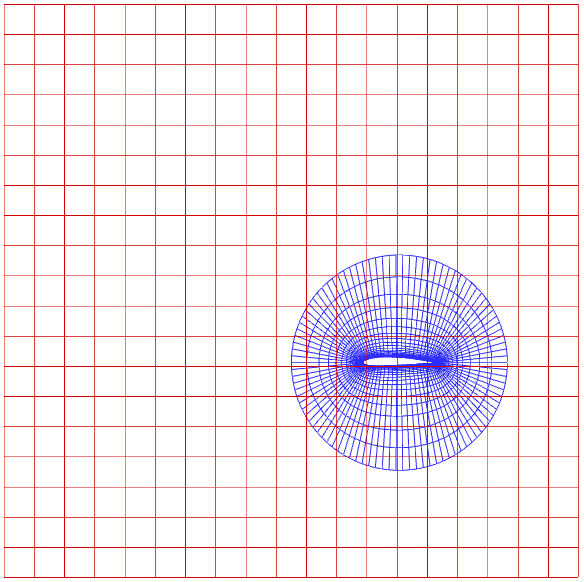
\includegraphics[width=0.3\linewidth]{figures/chimera_grid}
  \caption{Chimera, overlapping grid for moving airfoil simulation}
  \label{f:chimera_grid}
\end{figure}


\subsubsection{Motivation for efficient wall distance computation}
Traditionally, the wall distance calculation would be of little
importance from an efficiency perspective. In stationary grid
simulations, the wall distance does not change, and so it would only
be performed once as a pre-processing step, which would represent a
trivial amount of time compared to the overall calculation. For moving
body simulations however, the wall distance can change after each
update of the body position and thus has to be recomputed for every
iteration. It becomes extremely important then, to have an efficient
method for recomuting the wall distance in order to maintain
reasonable computation times. Using graphics processing units(GPU's)
to accelerate the wall distance computation is seen as a promising
method for improving computational efficiency for moving body
problems.

\section{Application-level objectives}
The goal for this project is to implement a parallel algorithm for
computing the wall distance for a computational grid on a GPU. The
benefit of implementing this portion of the CFD code will be improved
efficiency for moving body CFD calculations. In this investigation,
two primary methods will be investigated for computing the wall
distance field; a brute-force algorithm, and also an advancing
boundary algorithm. Each of these methods can be parallelized in a
number of different ways, and the details of each method along with
parallelization options will be discussed in detail. \\

Primary objectives:
\begin{itemize}
  \item Serial brute force wall distance calculation
  \item Parallel implementation of brute force method
\end{itemize}

Secondary objectives:
\begin{itemize}
  \item Serial implementation of advancing boundary algorithm
  \item Parallel implementation of advancing boundary algorithm
\end{itemize}

\section{Design overview}

\subsection{Preprocessor}
A preprocessor will be developed in order handle reading the computationsl grid and
formatting the data into an efficient manner for use by the wall
distance calculation algorithms. This module can be seen in block
diagram form in Figure~\ref{f:preprocessor_block}.

\begin{figure}
  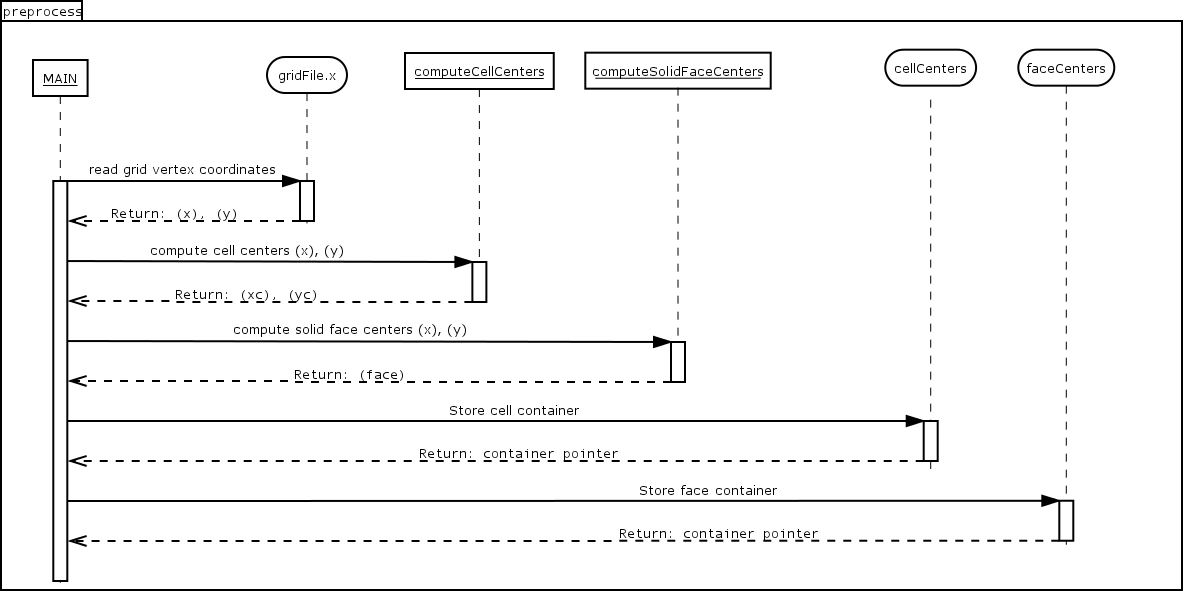
\includegraphics{figures/preprocessor/preprocessor_block}
  \caption{Block diagram for data preprocessor}
  \label{f:preprocessor_block}
\end{figure}


\subsection{Brute force algorithm}

\begin{figure}
  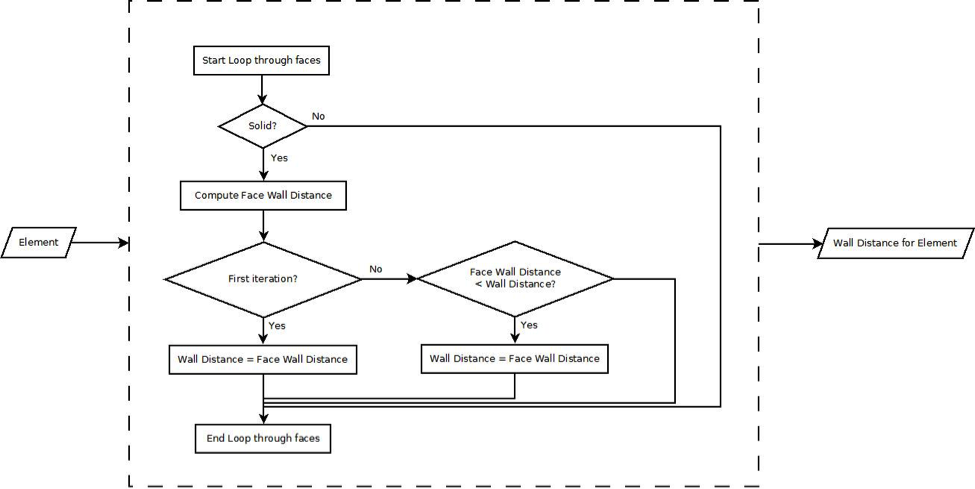
\includegraphics{figures/brute_force/bf_serial_block}
  \caption{Serial, brute force algorithm}
  \label{f:bf_serial}
\end{figure}

\subsubsection{Serial}
A serial brute-force implementation for calculating the wall distance
for an element is shown in Figure~\ref{f:bf_serial}. For each element, a large number of faces would have to be evaluated to check if the face is solid, to calculate its distance from the wall, and then to update the wall distance if this face has the least distance. The opportunity for parallelism arises in being able to perform the checks and wall distance calculation for each face separately.

For each face:
\begin{itemize}
  \item Wall distance from the face will be calculated
  \item b.	The minimum wall distance will be updated if the face wall distance is lower than the current minimum wall distance
\end{itemize}

In the worst case, work and step complexities for the serial approach
with n faces would be:

\begin{itemize}
  \item W ~ n*m = O(mn) – for each element, each solid face will have to be evaluated.  So, total number of operations is O(mn)
  \item S ~ m = O(m) – all the elements can be evaluated in parallel, but the distance from each solid face to the element is evaluated in sequence.  So, the longest chain of sequential dependencies is O(m).
\end{itemize}

\subsubsection{Parallel}

\begin{figure}
  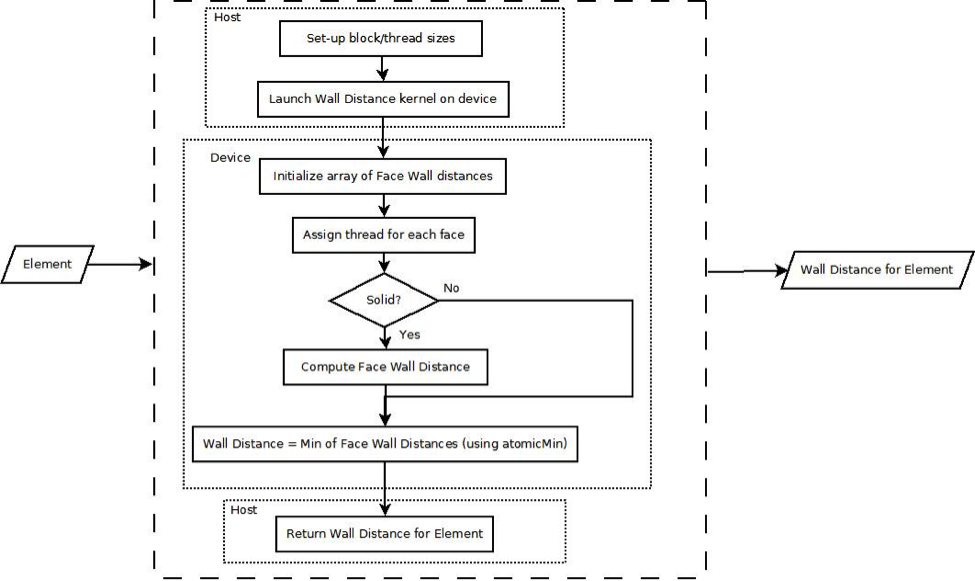
\includegraphics{figures/brute_force/bf_parallel1_block}
  \caption{Parallel, brute force algorithm \#1}
  \label{f:bf_parallel1}
\end{figure}

Two simple parallel implementations for the brute-force method will be explored.  The first parallel implementation for calculating the wall distance for an element is shown in Figure~\ref{f:bf_parallel1}.  For each element, the host sets up block and thread sizes, and then launches a device kernel.  The device kernel will assign a thread for each face, and then compute the wall distance for that face.  The minimum wall distance operation will be computed using atomic min so that only one thread is reading and updating the overall wall distance at a given time. 

The work complexity for this parallel implementation is similar to the
serial implementation:

\begin{itemize}
  \item W ~ n*m = O(mn).
\end{itemize}

It is slightly higher than the serial as there is additional overhead for assigning threads and initializing face wall distance in the parallel implementation.
Assuming infinite threads, the wall distances for each solid face can be calculated in parallel in one step.  However, the atomic min operation will limit the amount of parallelism that can be performed, as each thread may have to wait a long time before updating the minimum wall distance.  Though the step complexity for this parallel implementation can be improved by dividing the atomic operations to be within blocks, and then combining the results from the blocks, it will not be significantly better than the serial implementation:

\begin{itemize}
  \item S ~ m = O(m)
\end{itemize}


\begin{figure}
  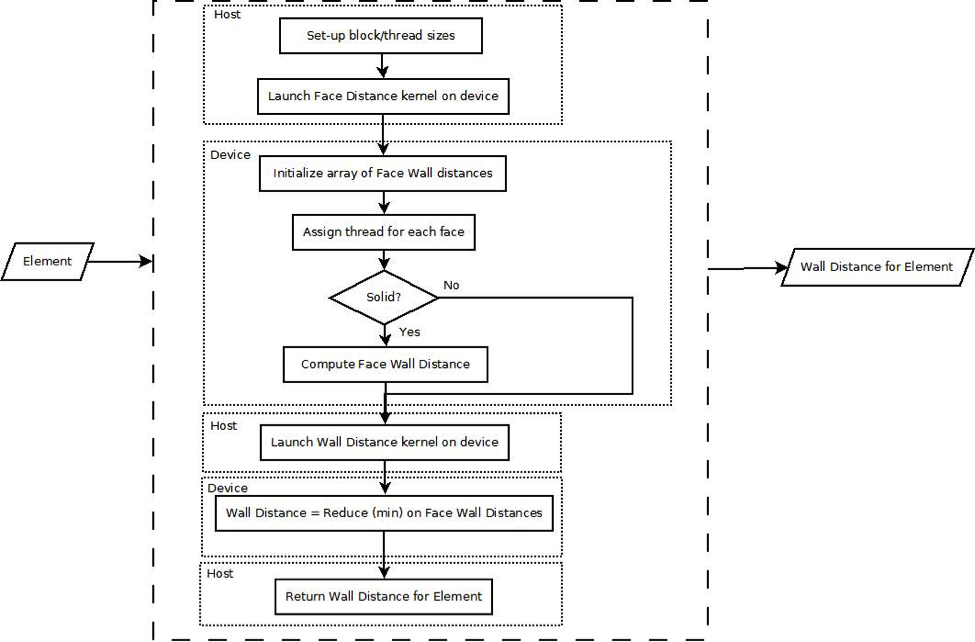
\includegraphics{figures/brute_force/bf_parallel2_block}
  \caption{Parallel, brute force algorithm \#2}
  \label{f:bf_parallel2}
\end{figure}

The second parallel implementation for calculating the wall distance for an element is shown in Figure~\ref{f:bf_parallel2}.  For each element, the host sets up block and thread sizes, and then launches device kernels.  The first kernel will assign a thread for each face, and then compute the wall distance for that face (same as the first parallel implementation).  However, after this kernel is executed, a reduce (minimum) operation will be performed to calculate the overall wall distance for the element, instead of using an atomic operation.  

The work complexity for this parallel implementation is similar to the first parallel (and serial) implementation:

\begin{itemize}
  \item W ~ n*m = O(mn)
\end{itemize}

However, the step complexity is much lower.  Assuming infinite threads, the wall distances for each face can be calculated in parallel in one step, and the reduce operation to compute the minimum wall distance has a step complexity of log m.  Therefore, step complexity for this parallel implementation is: 

\begin{itemize}
  \item S(n) ~ log m = O(log m).
\end{itemize}

\subsection{Advancing boundary algorithm}
The second method for computing the wall distance field for this
investigation is an advancing boundary algorithm that relies on creating an
auxiliary grid, which is used to identify a smaller subset of the
original set of solid faces that can be sorted more efficiently.

This method consists of two parts. First, a preprocessing step will be
used to compute an auxiliary grid overtop of the solid geometry. The
auxiliary grid will then be compacted to include only those cells
which intersect the solid boundary. The resulting auxiliary grid cells
should contain multiple geometry faces per cell in order to improve
efficiency. This auxiliary grid must would only be computed once at the
beginning of a CFD calculation, and so we are not concerned with the
efficiency of this step. A diagram of this process can be seen in
Figure~\ref{f:ab_preprocessor_diagram} but we are not concerned about
parallelizing this module.

\begin{figure}
  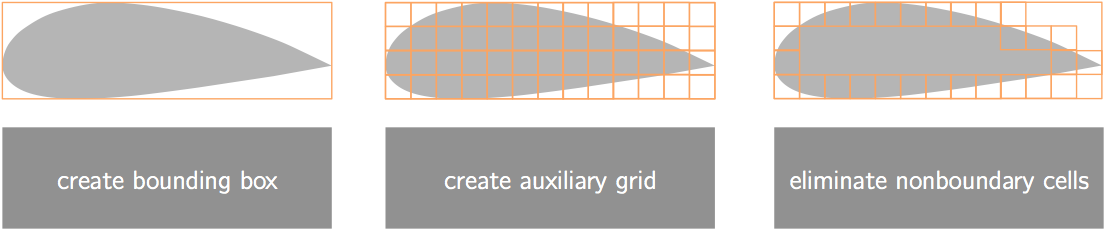
\includegraphics{figures/preprocessor/preprocessor_diagram}
  \caption{Advancing boundary method: preprocessing step}
  \label{f:ab_preprocessor_diagram}
\end{figure}


Once the preprocessing step is completed, the reduced auxiliary grid
is used as the input to the wall distance calculation. This process,
which was described above, can be seen in diagram form in
Figure~\ref{f:ab_diagram} and is used for each compuational cell in
the grid.


\begin{figure}
  \centering
  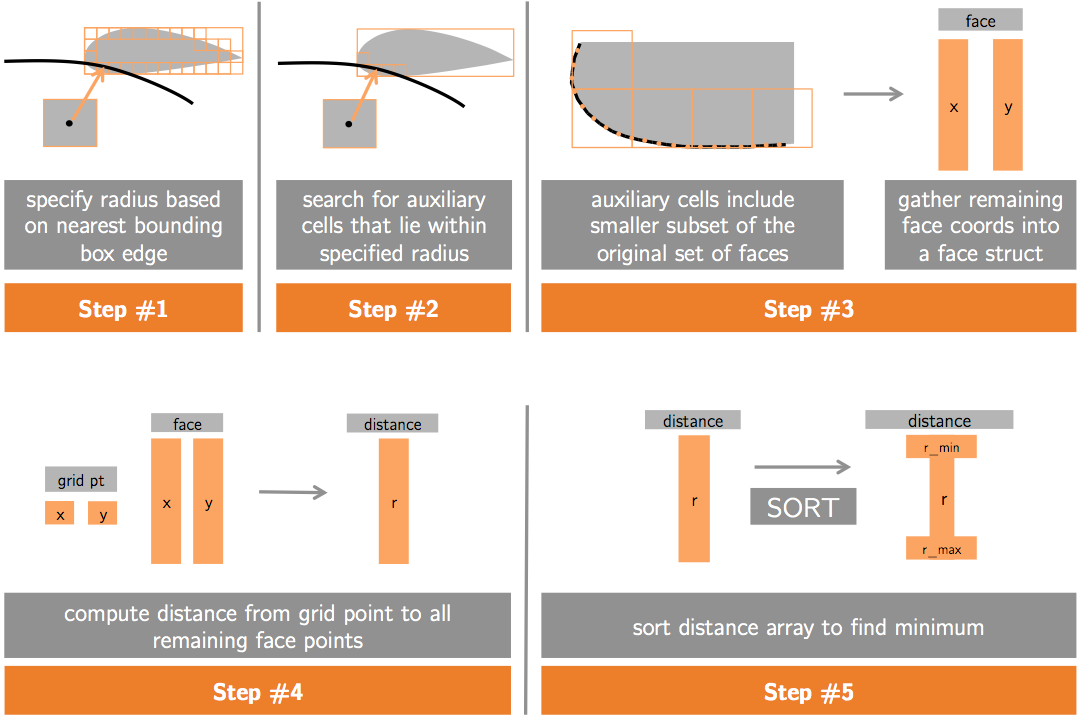
\includegraphics[width=0.95\linewidth]{figures/auxiliary_grid/algorithm_diagram}
\caption{Advancing boundary method: wall distance calculation}
\label{f:ab_diagram}
\end{figure}

\subsubsection{Parallelization}
There are several opportunities for potential gains in efficiency by
parallelizing certain portions of this algorithm. These opportunities
are outlined in the list below:

\begin{itemize}
\item Step \#2: Implement compact kernel to search for auxiliary cells
  that lie within specified radius. Returns array of remaining
  auxiliary cells.
  
\item Step \#4: Implement map kernel to compute remaining distance
  values. Returns array of wall distances.
  
\item Step \#5: Implement sort kernel to find minimum wall
  distance. Returns minimum wall distance.
\end{itemize}.

A block diagram of the algorithm is shown in
Figure~\ref{f:ag_block}. Additionally, a sequence diagram outlining
function/kernel calls is shown in Figure~\ref{f:ag_sequence}.

\begin{figure}
  \centering
  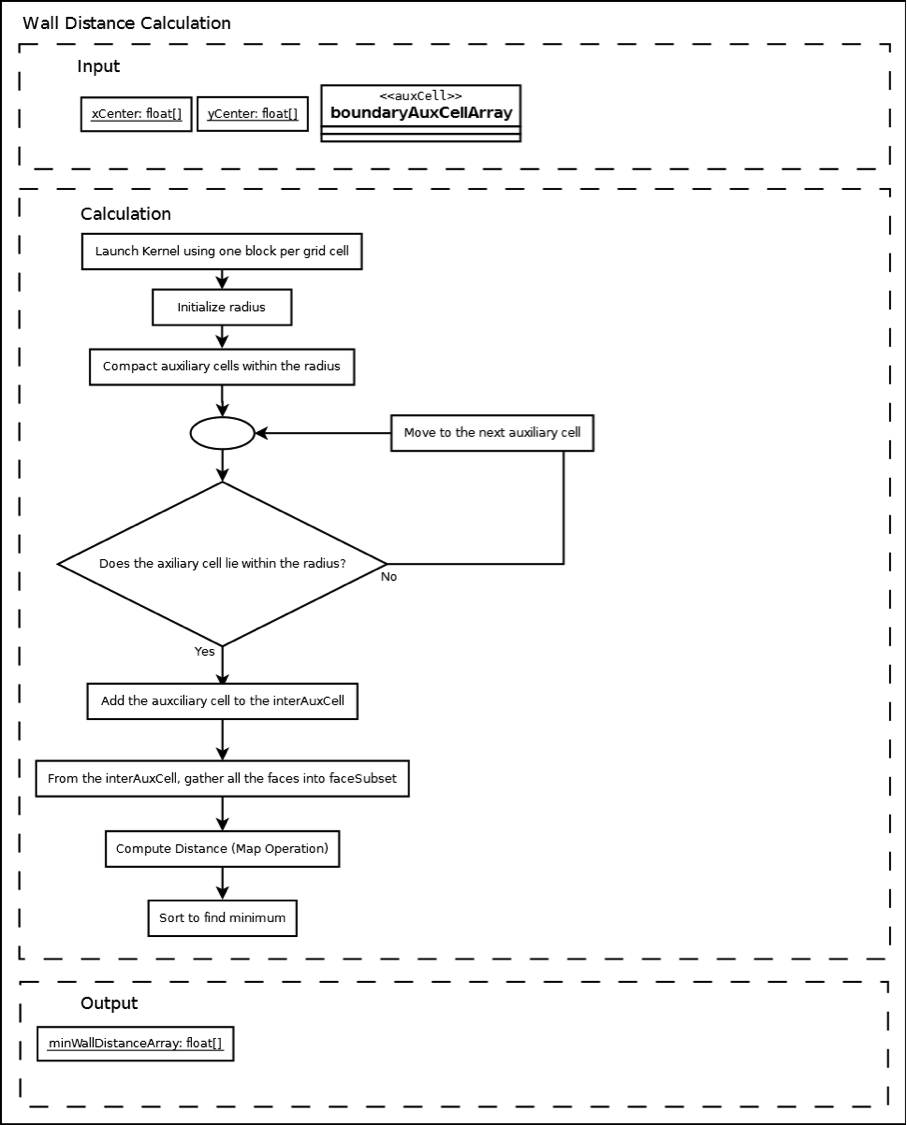
\includegraphics[width=0.7\linewidth]{figures/auxiliary_grid/ab_block}
  \caption{Auxiliary grid method: block diagram}
  \label{f:ag_block}
\end{figure}


\begin{figure}
  \centering
  \includegraphics[trim=0.0cm 11.0cm 0.0cm 0.0cm, clip=true, width=0.7\linewidth]{figures/auxiliary_grid/wallDistance_sequence}
  \caption{Ausiliary grid method: sequence diagram}
  \label{f:ag_sequence}
\end{figure}

\section{Performance goals}

\subsection{Brute force method}
The first parallel brute force implementation is not expected to have a significant impact on overall throughput, as the atomic min operation will limit the amount of parallelism that can be performed.  Each thread may have to wait a long time before updating the minimum wall distance.  However, the second parallel implementation is expected to complete execution in a much shorter time period than the serial implementation.  The speedup ratio is expected to be as close to m/(log m) as possible.  For example, if we have 65,536 solid faces, the second parallel implementation should be able to compute the wall distance in 16 steps, compared to 65,536 steps in the serial implementation. Potential bottlenecks for this performance goal are the number of blocks and threads available, and accessing global memory. In order to achieve the most efficient parallel implementation, several techniques will be explored such as assigning an efficient number of block and thread sizes, along with efficient memory usage such as coalesced memory access, and use of available shared memory and thread local memory.

\subsection{Advancing boundary method}
The advancing boundary method is largely experimental and it is
unclear at the moment if this method will improve efficiency due to
more kernel calls that would have to be executed. The efficiency will
also be dependent on the size of the problem and the ratio of solid
faces to grid cells. A study will be performed to evaluate the
trade-off between problem size and computational efficiency.

\subsection{Verification}
The verification of each algorithm will follow a visual method,
similar to the process used by the Udacity course. The wall distance
field variables will be stored to a file that can be opened along with
the computational grid to view the wall distance field. A visual
inspection is expected to be sufficient verification as any errors will
be easily detected.



\section{Schedule and division of work}
Figure~\ref{f:schedule} shows the proposed development schedule for
this effort along with the tentative work split between the team contributors.

\begin{figure}
  \centering
  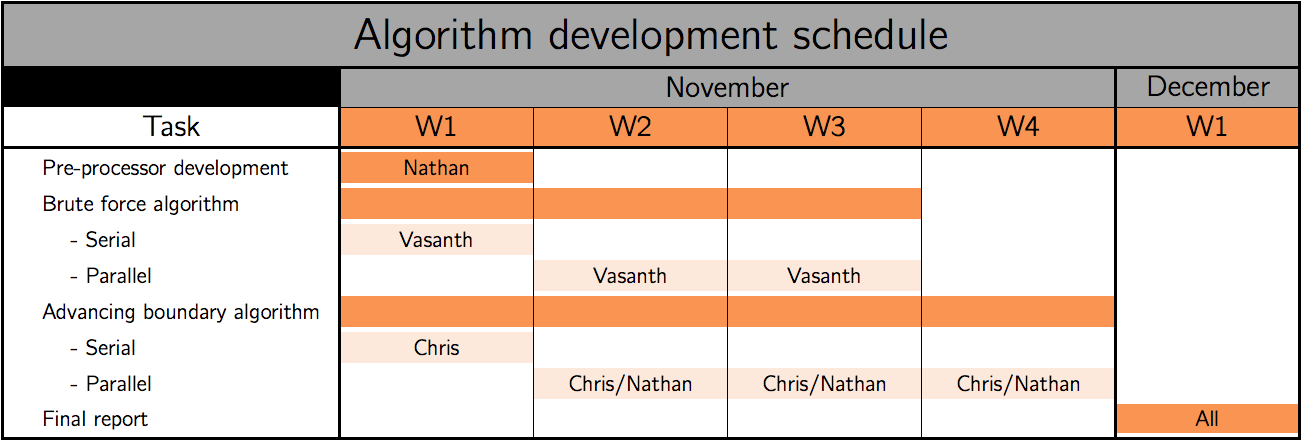
\includegraphics[width=0.9\linewidth]{figures/schedule}
  \caption{Development schedule and division of work}
  \label{f:schedule}
\end{figure}

% produces the bibliography section when processed by BibTeX
%\nocite{*}
%\bibliography{bibliography}
%\bibliographystyle{aiaa}

\end{document}

% - Release $Name:  $ -
